\documentclass{article}
\usepackage{hyperref, textcomp, pgfplots}
\pgfplotsset{width=7cm,compat=1.9}
\author{Samuel Havron \textlangle{}\href{mailto:havron@virginia.edu}{havron@virginia.edu}\textrangle{}}
\title{\textbf{Secure MPC as a Tool for Sensitive Data Analysis}}
\begin{document}
\maketitle
\section{Introduction}
A \emph{Secure multi-party computation} (MPC) is a protocol which allows for two or more parties to compute a function on sensitive input data provided by each party, without revealing anything about the inputs (other than what can be inferred from the revealed output result). 

Most current implementations of MPC work by executing instructions in a \emph{data-oblivious} manner, where the control flow of the program is independent of the inputs provided by each party and the program executes without any knowledge of the cleartext data it is operating on.  % may want some more details and cites here, explaining general-purpose MPC able to compute any function

%MPCs have practical uses for many organizations that have sensitive data sets which they cannot share, but could otherwise learn a lot by computing statistical functions on their joint data.
%For instance, two competitor companies may want to compute statistical functions on joint sales data and publish the results for internal company research and marketing, without allowing either competitor to uncover sensitive sales data about the other.
%In such situations it is important that neither company know the sales data inputs of their competitor, as they may learn secrets or be able to manipulate the data in their favor.
%By using an MPC protocol, the organizations can jointly compute functions of their combined sensitive data in such a manner that only the output of the program is revealed to them, with all sensitive input and intermediate results hidden. 


% replace the companies example with one more appropriate for social scientists -> see below


\begin{description}
\item[$\bullet$] Capabilities of MPC (including overview of previous work, Samee's implementation, efficiency/speed comparison with non-secure MPC programs) 
\item[$\bullet$] Value of MPC to social scientists, researchers (with motivating example(s)) as a tool for sensitive data analysis
\end{description}

% provides a motivating example for the usage of an MPC for social scientists and researchers

For instance, an education researcher may want to perform linear regression analysis on middle school students' GPAs and their family's income, without revealing any sensitive data about the students or their families. 
In one example, an education researcher may be interested in using statistical methods to analyze the relationship between a student's family income and the student's Grade Point Average for a particular school system or collection of school systems. Obtaining such sensitive data ... (* reference to CMU 2009 paper *)

% precision vs range
% examples of interesting linear regression

% matching records. big cost to researchers . 

% is there an identiifer field linked with both data values? e.g. a name or idenitifying number.
% could datasets be linked up by regex match?  


\section{Methods}
\begin{description}
\item[$\bullet$] Description of OblivC’s efficiency/speed in comparison to other existing MPC implementations
\item[$\bullet$] Overview of OblivC as a language, relationship to C (appeal to researchers with some C/basic programming experience) 
\item[$\bullet$] Introduce implementation of linear regression analysis program, use code snippets and reference repo/site tutorial
\end{description}
\section{Results}
\begin{description}
\item[$\bullet$] Discuss efficiency/speed/scalability of aforementioned linear regression analysis program, provide EC2 testing data (collect more formally prior to including in final paper). Mention single-threaded implementation and limits on performance results.
\item[$\bullet$] Discuss results of other motivating OblivC programs, compare to alternative MPC results
\end{description}

The scalability and speed of OblivC as a tool for implementing MPC programs was tested using c4.large \emph{Elastic Compute Cloud} (EC2) nodes from \emph{Amazon Web Services} (AWS) of Amazon.com\textregistered. Two c4.large instances were launched and connected through OblivC's API for TCP/IP connections. One node instance provided independent ($x$) data points, while the other provided dependent ($y$) data points. Data points used were 32-bit integers. Data for computation was mined from New York public health data (include link), as well as synthetic data points generated through a Python program (footnote for file location) for performance results.

\begin{center}
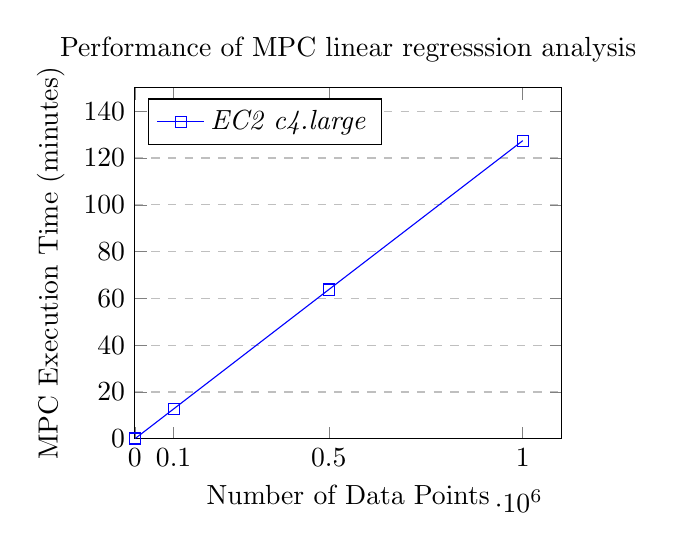
\begin{tikzpicture}
\begin{axis}[
    title={Performance of MPC linear regresssion analysis},
    xlabel={Number of Data Points},
    ylabel={MPC Execution Time (minutes)},
    xmin=0, xmax=1100000,
    ymin=0, ymax=150,
    xtick={0,100000,500000,1000000},
    ytick={0,20,40,60,80,100,120,140},
    legend pos=north west,
    ymajorgrids=true,
    grid style=dashed,
]
 
\addplot[
    color=blue,
    mark=square,
    ]
    coordinates {
    (1000,0.1088522)(100000,12.74658383)(500000,63.765116616)(1000000,127.42427975)
    };
    \legend{\emph{EC2 c4.large}}
 
\end{axis}
\end{tikzpicture}
\end{center}

% Does your implementation use multiple threads? The main difference between the EC2 nodes is the number of cores you are getting (as well as memory size), but if the implementation is only using 1 core, this won't make a difference.

% what does "input size" mean here?  is it the number of data points?  how big is each data point?

% time is clock time to complete protocol execution between two EC2 nodes?



\begin{description}
\item[$\bullet$] Include table with times from NY public health dataset computation.
\item[$\bullet$] Include table with times from non secure MPC computation for comparison.
\end{description}
\section{Conclusion}
\begin{description}
\item[$\bullet$] Overview of secure MPC, utility/extensibility of OblivC programming, real-world usage for scientists/researchers
\end{description}

A secure MPC ensures that only the result of data analysis on sensitive inputs is revealed. OblivC implements this under-the-hood using manipulations of Yao's Garbled
Circuits Protocol (* link to Samee's paper *).

Using OblivC as a tool to analyze real, sensitive data-sets requires only a basic understanding of the C programming language, and enthusiasm for experimenting with new API that
OblivC provides. A full tutorial for how to get started and an API documentation are available online (* update with link *). One particular aspect of OblivC in its current release is the lack of native
support for oblivious-qualified floating point numbers. A workaround using fixed point numbers is detailed in the linear regression example, specifically here (* update with link *). Preliminary work has been included in the code repository (* link *) for automating a data-matching process between two datasets, where a common identifier for data values (e.g. SSN) is mapped and party inputs are
matched up with a private set intersection protocol; researchers may find modifications to this source code useful in creating their own secure MPC applications for matching sensitive datasets
with a common identifier. 



\begin{thebibliography}{9} % include more references for later use

\bibitem{Lindell2009}
  Yehuda Lindell and Benny Pinkas,
  \emph{Secure Multiparty Computation for
Privacy-Preserving Data Mining},
  The Journal of Privacy and Confidentiality (2009),
  Number 1, pp. 59–98. Retrieved from \href{http://repository.cmu.edu/cgi/viewcontent.cgi?article=1004\&context=jpc}{http://repository.cmu.edu/cgi/viewcontent.cgi?article=1004\&context=jpc}. 

\end{thebibliography}
\end{document}
